\documentclass[10pt,notes,compress,usetitleprogressbar,aspectratio=1610]{beamer}

\usepackage[english]{babel}
\usepackage[T1]{fontenc}
\usepackage[utf8x]{inputenc}
\usepackage[caption=false,font=footnotesize]{subfig} 		% Separar figuras en subfiguras

\usepackage{/home/vicdejuan/Imdea-S/tfg/definitions}

\newcommand{\pc}{\ensuremath{\mathit{pc}}\xspace}

\definecolor{palette1}{HTML}{1B9E77}
\definecolor{palette2}{HTML}{D95F02}
\definecolor{palette3}{HTML}{7570B3}
\definecolor{palette4}{HTML}{E7298A}
\definecolor{palette5}{HTML}{66A61E}
\definecolor{palette6}{HTML}{E6AB02}
\definecolor{palette7}{HTML}{A6761D}
\definecolor{palette8}{HTML}{666666}

\usetheme{metropolis}



\usepackage{tikz}
\usepackage{tikztools}
\usetikzlibrary{calc,shapes.multipart,chains,arrows,tikzmark,fit,shapes.geometric}



\title{First Order Proofs for Concurrent Programs}
\subtitle{Bachelor thesis | Double Degree Computer Science and Mathematics}
\author{Víctor de Juan Sanz}
\date{July 2016}
\institute{Imdea Software}

\setbeameroption{hide notes}
%\setbeameroption{show notes}
% \setbeameroption{show only notes}


\newcommand{\PROGRAM}{\begin{array}{l@{\hspace{0.3em}}c@{\hspace{1em}}l}
		\hline
			l_1 & : & \mathtt{x := 10} \\
			l_2 & : & \mathtt{f := 1} \\
			l_3 & : & \mathtt{\textbf{while } (x\geq 1) \textbf{ do }} \\
			l_4 & : & \mathtt{\;\;f = f*x} \\
			l_5 & : & \mathtt{\;\;x=x-1} \\ 	
			l_6 & : & \mathtt{\textbf{end while}}\\
			l_7 & : & \mathtt{\cdots}\\
		\hline
		\end{array}}



\newcommand{\GOALS}{\varphi_1 \equiv \forall T([\pc(T) = l_5 \orcond \pc(T) = l_4 ]\to \mathtt{x}\geq 1) \;\; \wedge \;\; \varphi_2 \equiv \mathtt{x} \geq 0}

\newcommand{\TRANSITIONS}{	\begin{array}{l}
		 \tau_1 \equiv\pc(T) = l_1 \andcond \pc\prime (T) = l_2 \andcond \mathtt{f\prime =f} \andcond \mathtt{x}\prime  = 10\\
		 \tau_2 \equiv\pc(T) = l_2 \andcond \pc\prime (T) = l_3 \andcond \mathtt{f}\prime  = 1 \andcond x\prime =x\\
		 \tau_3 \equiv\pc(T) = l_3 \andcond \pc\prime (T) = l_4 \andcond \mathtt{f\prime =f} \andcond x\prime \geq 1\\
		 \tau_4 \equiv\pc(T) = l_4 \andcond \pc\prime (T) = l_5 \andcond \mathtt{f}\prime  = \mathtt{f*x} \andcond \mathtt{x\prime =x}\\
		 \tau_5 \equiv\pc(T) = l_5 \andcond \pc\prime (T) = l_3 \andcond \mathtt{f\prime =f} \andcond \mathtt{x\prime =x-1}\\
		 \tau_6 \equiv\pc(T) = l_3 \andcond \pc\prime (T) = l_7 \andcond \mathtt{f\prime =f} \andcond \mathtt{x<1}
	\end{array}}



\renewcommand{\formulaFullListReducedBody}{
  \left\{
    \begin{array}{llc}
      \fNull \in \region \andcond
      \region = \fAddrToSet(\heap, \head) \andcond
      \head \neq \tail & \andcond & \text{(L1)} \\
      \heap[\tail].\fNext = \fNull \andcond
      \tail \neq \fNull \andcond
      \head \neq \fNull & \andcond & \text{(L2)} \\
      \heap[\head].\fData = -\infty \andcond
      \heap[\tail].\fData = +\infty & \andcond & \text{(L3)} \\
			\Ordered (\heap, \head, \tail) && \text{(L4)}
    \end{array}
  \right.
 }


\begin{document}

\begin{frame}
\end{frame}

\maketitle

\begin{frame}{Table of contents}
	\begin{center}
		\setbeamertemplate{section in toc}[sections numbered]
		\tableofcontents[hideallsubsections]
	\end{center}
\end{frame}

%%%%%%%%%%%%%%%%%%%%%%%%%%%%%%%%%%%%%%%%%%%%%%%%%%%%%%%%%%%%%%%%%%%%%%
%%%%%%%%%%%%%%%%%%%%%%%%%%%%%%%%%%%%%%%%%%%%%%%%%%%%%%%%%%%%%%%%%%%%%%
%%%%%%%%%%%%%%%%%%%%		Motivation 			%%%%%%%%%%%%%%%%%%%%%%
%%%%%%%%%%%%%%%%%%%%%%%%%%%%%%%%%%%%%%%%%%%%%%%%%%%%%%%%%%%%%%%%%%%%%%
%%%%%%%%%%%%%%%%%%%%%%%%%%%%%%%%%%%%%%%%%%%%%%%%%%%%%%%%%%%%%%%%%%%%%%

\section{Motivation}

\begin{frame}{Motivation}
	\begin{figure}
		\centering
		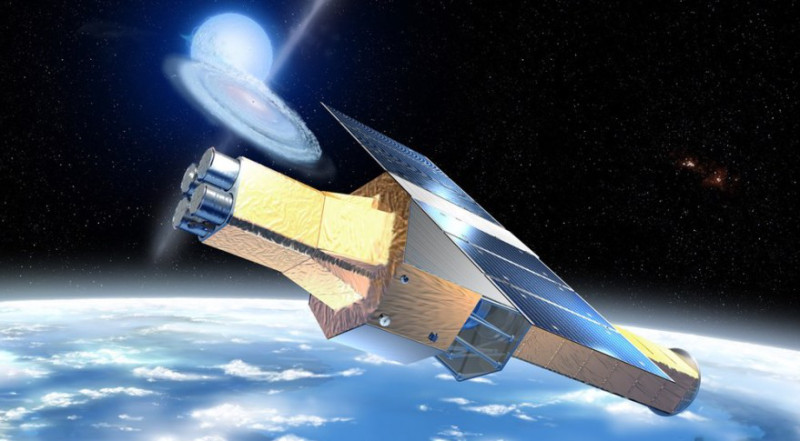
\includegraphics[scale=0.4]{imgs/japanesse.jpg}
		\caption{Japanese satellite lost in space: \$248 million.}
	\end{figure}
\end{frame}

\begin{frame}{Motivation}
	\begin{figure}
		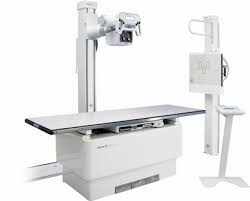
\includegraphics[scale=0.9]{imgs/xray.jpg}
		\caption{XRay machine: Between 1985 and 1987 6 people died.}
	\end{figure}
\end{frame}

\begin{frame}{Motivation}
	\begin{figure}
		\centering
		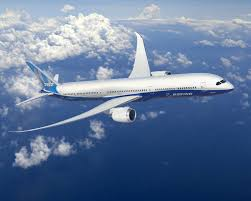
\includegraphics[scale=0.8]{imgs/boeing.jpg}
		\caption{Boeing 787: \textit{failsafe} mode.}
	\end{figure}
\end{frame}

\section{Objectives}

\begin{frame}{Objectives}
\begin{itemize}
	\item Prove correctness of an implementation of an ordered linked list.
	\begin{itemize}
		\item[--] Preservation as a list and order preservation.
	\end{itemize}
	\begin{figure}
		\newcommand{\Cross}{$\mathbin{\tikz [x=1.4ex,y=1.4ex,line width=.2ex, red] \draw (0,0) -- (1,1) (0,1) -- (1,0);}$}%

\newcommand{\Checkmark}{$\color{green}\checkmark$}


	\subfloat{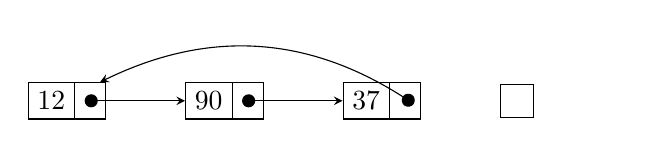
\begin{tikzpicture}[list/.style={rectangle split, rectangle split parts=2,draw, rectangle split horizontal}, >=stealth, start chain]
		  \node[list,on chain] (A) {12};
		  \node[list,on chain] (B) {90};
		  \node[list,on chain] (C) {37};
		  \node[on chain,draw,inner sep=6pt] (D) {$\fNull$};
		  \node at (7,0) (T) {\LARGE\Cross};
		  \draw[*->] let \p1 = (A.two), \p2 = (A.center) in (\x1,\y2) to (B);
		  \draw[*->] let \p1 = (B.two), \p2 = (B.center) in (\x1,\y2) to (C);
		  \draw[*->] let \p1 = (C.two), \p2 = (C.center) in (\x1 + 5.1,\y2-1.1) to[bend right] (A);
	\end{tikzpicture}}
	
	\vspace{0.4cm}

		\subfloat{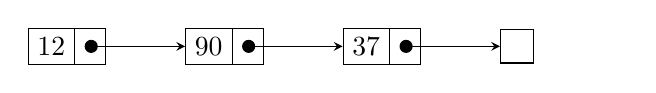
\begin{tikzpicture}[list/.style={rectangle split, rectangle split parts=2,draw, rectangle split horizontal}, >=stealth, start chain]
		  \node[list,on chain] (A) {12};
		  \node[list,on chain] (B) {90};
		  \node[list,on chain] (C) {37};
		  \node[on chain,draw,inner sep=6pt] (D) {$\fNull$};
		  \node at (7,0) (T) {\LARGE\Cross};
		  \draw[*->] let \p1 = (A.two), \p2 = (A.center) in (\x1,\y2) -- (B);
		  \draw[*->] let \p1 = (B.two), \p2 = (B.center) in (\x1,\y2) -- (C);
		  \draw[*->] let \p1 = (C.two), \p2 = (C.center) in (\x1,\y2) -- (D);
	\end{tikzpicture}}
	
	\vspace{0.4cm}

		\subfloat{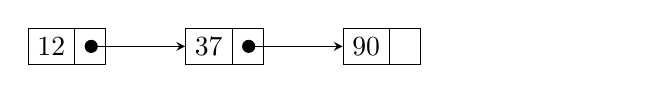
\begin{tikzpicture}[list/.style={rectangle split, rectangle split parts=2,draw, rectangle split horizontal}, >=stealth, start chain]
		  \node[list,on chain] (A) {12};
		  \node[list,on chain] (B) {37};
		  \node[list,on chain] (C) {90};
		  \node at (7,0) (T) {\LARGE\Cross};
		  \draw[*->] let \p1 = (A.two), \p2 = (A.center) in (\x1,\y2) -- (B);
		  \draw[*->] let \p1 = (B.two), \p2 = (B.center) in (\x1,\y2) -- (C);
	\end{tikzpicture}}
	
	\vspace{0.4cm}

	\subfloat{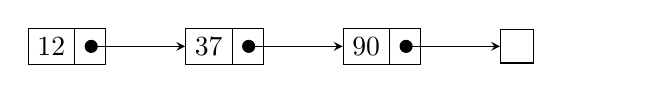
\begin{tikzpicture}[list/.style={rectangle split, rectangle split parts=2,draw, rectangle split horizontal}, >=stealth, start chain]
		  \node[list,on chain] (A) {12};
		  \node[list,on chain,bend right] (B) {37};
		  \node[list,on chain] (C) {90};
		  \node[on chain,draw,inner sep=6pt] (D) {$\fNull$};
		  \node at (7,0) (T) {\LARGE\Checkmark};
		  \draw[*->] let \p1 = (A.two), \p2 = (A.center) in (\x1,\y2) -- (B);
		  \draw[*->] let \p1 = (B.two), \p2 = (B.center) in (\x1,\y2) -- (C);
		  \draw[*->] let \p1 = (C.two), \p2 = (C.center) in (\x1,\y2) -- (D);
	\end{tikzpicture}}
	\end{figure}
	\item[]
	\item[]
\end{itemize}
\end{frame}

\begin{frame}{Objectives}
\begin{itemize}
	\item Prove correctness of an implementation of an ordered linked list.
	\begin{itemize}
		\item[--] Preservation as a list and order preservation.
	\end{itemize}
	\begin{figure}
		\newcommand{\Cross}{$\mathbin{\tikz [x=1.4ex,y=1.4ex,line width=.2ex, red] \draw (0,0) -- (1,1) (0,1) -- (1,0);}$}%

\newcommand{\Checkmark}{$\color{green}\checkmark$}


	\subfloat{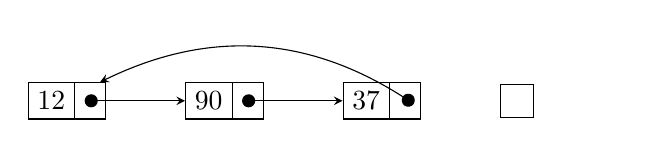
\begin{tikzpicture}[list/.style={rectangle split, rectangle split parts=2,draw, rectangle split horizontal}, >=stealth, start chain]
		  \node[list,on chain] (A) {12};
		  \node[list,on chain] (B) {90};
		  \node[list,on chain] (C) {37};
		  \node[on chain,draw,inner sep=6pt] (D) {$\fNull$};
		  \node at (7,0) (T) {\LARGE\Cross};
		  \draw[*->] let \p1 = (A.two), \p2 = (A.center) in (\x1,\y2) to (B);
		  \draw[*->] let \p1 = (B.two), \p2 = (B.center) in (\x1,\y2) to (C);
		  \draw[*->] let \p1 = (C.two), \p2 = (C.center) in (\x1 + 5.1,\y2-1.1) to[bend right] (A);
	\end{tikzpicture}}
	
	\vspace{0.4cm}

		\subfloat{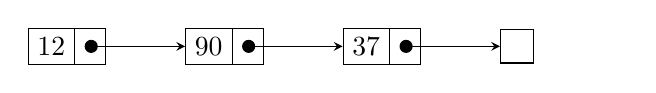
\begin{tikzpicture}[list/.style={rectangle split, rectangle split parts=2,draw, rectangle split horizontal}, >=stealth, start chain]
		  \node[list,on chain] (A) {12};
		  \node[list,on chain] (B) {90};
		  \node[list,on chain] (C) {37};
		  \node[on chain,draw,inner sep=6pt] (D) {$\fNull$};
		  \node at (7,0) (T) {\LARGE\Cross};
		  \draw[*->] let \p1 = (A.two), \p2 = (A.center) in (\x1,\y2) -- (B);
		  \draw[*->] let \p1 = (B.two), \p2 = (B.center) in (\x1,\y2) -- (C);
		  \draw[*->] let \p1 = (C.two), \p2 = (C.center) in (\x1,\y2) -- (D);
	\end{tikzpicture}}
	
	\vspace{0.4cm}

		\subfloat{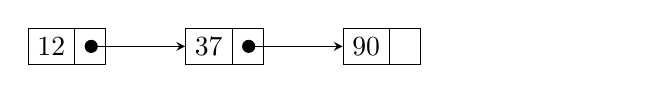
\begin{tikzpicture}[list/.style={rectangle split, rectangle split parts=2,draw, rectangle split horizontal}, >=stealth, start chain]
		  \node[list,on chain] (A) {12};
		  \node[list,on chain] (B) {37};
		  \node[list,on chain] (C) {90};
		  \node at (7,0) (T) {\LARGE\Cross};
		  \draw[*->] let \p1 = (A.two), \p2 = (A.center) in (\x1,\y2) -- (B);
		  \draw[*->] let \p1 = (B.two), \p2 = (B.center) in (\x1,\y2) -- (C);
	\end{tikzpicture}}
	
	\vspace{0.4cm}

	\subfloat{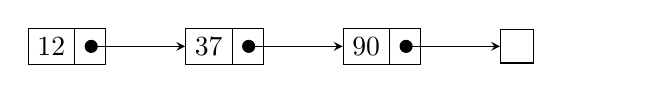
\begin{tikzpicture}[list/.style={rectangle split, rectangle split parts=2,draw, rectangle split horizontal}, >=stealth, start chain]
		  \node[list,on chain] (A) {12};
		  \node[list,on chain,bend right] (B) {37};
		  \node[list,on chain] (C) {90};
		  \node[on chain,draw,inner sep=6pt] (D) {$\fNull$};
		  \node at (7,0) (T) {\LARGE\Checkmark};
		  \draw[*->] let \p1 = (A.two), \p2 = (A.center) in (\x1,\y2) -- (B);
		  \draw[*->] let \p1 = (B.two), \p2 = (B.center) in (\x1,\y2) -- (C);
		  \draw[*->] let \p1 = (C.two), \p2 = (C.center) in (\x1,\y2) -- (D);
	\end{tikzpicture}}
	\end{figure}
	\item  Formal verification of the correctness.
	\item Concurrent linked list (fine grain lock couple)
\end{itemize}
\end{frame}

\section{Preliminaries}

\begin{frame}{Preliminaries}
\begin{itemize}
	\item We assume the usual way of representing and working with First Order Logic (FOL)
	%\item Formal verification is proving correctness.... \textcolor{red}{LoL}
	\item We approach to assess correctness is by proving properties:
	\begin{itemize}
		\item \tikzmark{start1}Safety properties.\tikzmark{end1}
		\item Lifeness properties.
		\item Functional properties.
	\end{itemize}
	\begin{tikzpicture}[remember picture,overlay]
		\node<2,3>[draw,line width=2pt,orange,ellipse,inner ysep=8pt,fit={(pic cs:start1) (pic cs:end1)}] {};
		\node<3>[draw] at (5,1.5) {$\mathtt{x}≠0$};
	\end{tikzpicture} 
\end{itemize}
\end{frame}

\subsection{Simple Programming Language (SPL)}

\begin{frame}{Simple Programming Language (SPL)}
\note{\begin{itemize}
	\item Pre-estado y postestado.
\end{itemize}}
\[
	\begin{array}[t]{ll}
		\hline
		\text{Statement} & \text{Transition relation} \\ \hline\hline
		\begin{array}[t]{l@{\hspace{0.3em}}c@{\hspace{1em}}l}
			\ell_1 & : & \mathtt{\textbf{while } c \textbf{ do }} \\
			\ell_2 & : & \mathtt{\cdots} \\
			\mathtt{\vdots} \\
			\ell_n & : & \mathtt{\textbf{end while}} \\
			\ell_{n+1} & : & \mathtt{\cdots}
		\end{array}
		&
		\begin{array}[t]{ll}
				(\pc(T) = \ell_1 \andcond \;\;\texttt{c} \andcond \pc'(T) = \ell_2) \; 
				\orcond \\
				(\pc(T) = \ell_1 \andcond \lnot \texttt{c} \andcond \pc'(T) = 
			\ell_{n+1})
			& \text{for line $\ell_1$} \\ \\
			\pc(T) = \ell_n \andcond \pc'(T) = \ell_1 &
				\text{for line $\ell_n$}
		 \end{array} \\ \hline
	 \end{array}
\]
\end{frame}

\subsection{Inductive Assertion Method}
\begin{frame}{Inductive Assertion Method}
\note{\begin{itemize}
	\item Un programa no concurrente, por ser un ejemplo más ilutrativo. 
	\item El objetivo es probar que hay fórmulas \textbf{invariantes}. 
	\item Es fácil ver que esto es cierto, tal y como lo tenemos aquí. Ilustramos el método con un ejemplo simple para que se entienda bien.
\end{itemize}}

	\begin{block}<1->{}
		\begin{center}
			\vspace{-1cm}
			\[
				\PROGRAM
			\]
		\end{center}
	\end{block}

	\begin{block}<2>{}
		\begin{center}
			
			\[
				\GOALS
			\]
		\end{center}
	\end{block}

	\begin{block}<3->{}
		\begin{center}
		\vspace{-4cm}
			\[
				\TRANSITIONS
			\]
		\end{center}
	\end{block}
\end{frame}


\begin{frame}{Inductive Assertion Method}
\note{\begin{itemize}
	\item En naranja, las condiciones de verificación.
	\item Si todas las condiciones de verificación son válidas, el candidato a invariante es un invariante.
\end{itemize}}
	\[
		\left.
			\begin{array}{ll}
				\textbf{Program:} 		&	 \PROGRAM \\\\
				\textbf{Transitions:}	&	 \TRANSITIONS \\\\
				\textbf{Goal : }	 	&	 \GOALS
			\end{array}
		\right\}
		\tikzmark{start2}
		\begin{array}{l}
			\text{VCs:}
			\\
			\begin{array}{r}
				\theta \to \varphi_i\;							\\
				\tau_1 \andcond \varphi_i \to \varphi_i\prime	\\
				\tau_2 \andcond \varphi_i \to \varphi_i\prime 	\\
				\tau_3 \andcond \varphi_i \to \varphi_i\prime	\\
				\tau_4 \andcond \varphi_i \to \varphi_i\prime	\\
				\tau_5 \andcond \varphi_i \to \varphi_i\prime	\\
				\tau_6 \andcond \varphi_i \to \varphi_i\prime 
			\end{array}
		\end{array}
		\tikzmark{end2}
	\]
	\begin{tikzpicture}[remember picture,overlay]
		\node<2>[draw,line width=2pt,orange,square,inner ysep=64pt,fit={(pic cs:start2) (pic cs:end2)}] {};
	\end{tikzpicture} 

\end{frame}


\begin{frame}{Inductive Assertion Method}
	\paragraph{Some proofs for the invariance of $\varphi_1$:}
	\note{
	\begin{itemize}
		\item 1: Una cualquiera.
		\item 2: Claro, la interesante será en la que se modifica el valor de la x.
		\item 3: No, la interesante es la que llega a esa línea.
	\end{itemize}
	}

%	\only<1>{\begin{block}{}
%		 $\tau_2 \andcond \varphi_1 \to \varphi_1\prime $:
	%	\begin{dmath*}[indentstep={0em}]
%		\begin{align*}
%			(
%				\underbrace{\textcolor{black}{\pc(T) = l_2} \andcond \textcolor{orange}{\pc\prime (T) = l_3} \andcond \mathtt{f}\prime  = 1 \andcond x\prime =x}_{\tau_2} \andcond (\underbrace{[\textcolor{black}{\pc(T) = l_5 \orcond \pc(T) = l_4 }] \to \mathtt{x}\geq 1}_{\varphi_1})
%			) \\
%				\to(\underbrace{[\textcolor{orange}{\pc\prime (T) = l_5 \orcond \pc\prime(T) = l_4}] \to \mathtt{x}\prime  \geq 1}_{\varphi_1\prime })\;\;\;\;
%		\end{align*}
%	\end{block}}

	\only<1>{
	\begin{block}{}
	 	$\tau_5 \andcond \varphi_1 \to \varphi_1\prime $:
	%	\begin{dmath*}[indentstep={0em}]
		\begin{align*}
			(
				\underbrace{\pc(T) = l_5 \andcond \textcolor{orange}{\pc\prime (T) = l_3} \andcond \mathtt{f\prime =f} \andcond \mathtt{x\prime =x-1}}_{\tau_5} \andcond (\underbrace{[\pc(T) = l_5 \orcond \pc(T) = l_4] \to \mathtt{x}\geq 1}_{\varphi_1})
			) \\
				\to(\underbrace{[\textcolor{orange}{\pc\prime (T) = l_5 \orcond \pc\prime(T) = l_4 }] \to \mathtt{x}\prime  \geq 1}_{\varphi_1\prime })\;\;\;\;
		\end{align*}
	\end{block}}

	\only<2>{\begin{block}{}
		 \;$\tau_4 \andcond \varphi_1 \to \varphi_1\prime $: 
		\begin{align*}
			(
				\underbrace{\textcolor{cyan}{\pc(T) = l_4} \andcond \textcolor{orange}{\pc\prime (T) = l_5} \andcond \mathtt{f}\prime  = \mathtt{f*x} \andcond \mathtt{x\prime =x}}_{\tau_4} \andcond (\underbrace{[\pc(T) = l_5 \orcond \textcolor{cyan}{\pc(T) = l_4}]  \to \mathtt{x}\geq 1}_{\varphi_1})
			) \\
				\to(\underbrace{[\textcolor{orange}{\pc\prime (T) = l_5 \orcond \pc\prime(T) = l_4 }] \to \mathtt{x}\prime  \geq 1}_{\varphi_1\prime })\;\;\;\;
		\end{align*}
		Equivalent to:
		\begin{equation*}
			(
				\mathtt{x\prime =x} \andcond  \mathtt{x}\geq 1
			) 
			\to (\mathtt{x}\prime \geq 1)
		\end{equation*}
	\end{block}}



\end{frame}

\begin{frame}{Inductive Assertion Method}
	\paragraph{Conclusion:}
		\begin{itemize}
			\item $\varphi_1$ is an \textbf{inductive invariant}.
		\end{itemize}
\end{frame}

\begin{frame}{Inductive Assertion Method}
	\paragraph{One proof for the invariance of $\varphi_2$:}

	\; $\tau_5 \andcond \varphi_2 \to \varphi_2\prime $:	
%	\begin{dmath*}[indentstep={0em}]
	\begin{equation*}
		(
			\underbrace{\pc(T) = l_5 \andcond \pc\prime (T) = l_3 \andcond \mathtt{f\prime =f} \andcond \mathtt{x\prime =x-1}}_{\tau_5} \andcond \underbrace{\mathtt{x} \geq 0}_{\varphi_2}
		) 
			\to \underbrace{\mathtt{x}\prime  \geq 0}_{\varphi_2\prime }\\\\
	\end{equation*}

	\only<2>{\begin{block}{}
		\begin{center}\textcolor{red}{\textbf{Counter example:}} $x=0$\end{center}
	\end{block}}
	\only<3>{\begin{block}{}
		\begin{center}$\varphi_1 \equiv \pc(T) = l_5 \to x ≥ 1$. Can we use that information?\end{center}
	\end{block}}
\end{frame}

\begin{frame}{Inductive Assertion Method}
	\textbf{Support:}


	\[
		(\tau_5 \andcond \textcolor{orange}{\varphi_1} \andcond \varphi_2 \to \varphi_2\prime ) \rightarrow ( \tau_5 \andcond \varphi_2\to\varphi_2\prime )
	\]

	\begin{block}<2->{}
	\vspace{-1cm}
		\textbf{We prove:}
		\begin{equation*}
			(
				\underbrace{\pc(T) = l_5 \andcond \pc\prime (T) = l_3 \andcond \mathtt{f\prime =f} \andcond \mathtt{x\prime =x-1}}_{\tau_5} \andcond \underbrace{\mathtt{x} \geq 0}_{\varphi_2} \andcond \underbrace{\pc(T) = l_5 \to \mathtt{x} \geq 1}_{\varphi_1}
			) 
				\to \underbrace{\mathtt{x}\prime  \geq 0}_{\varphi_2\prime }\\\\
		\end{equation*}
	\end{block}

	\only<3>{\begin{block}{}
		\vspace{-1cm}
		\textbf{Equivalent to:}
		\[
			( \mathtt{x\prime =x-1} \andcond \mathtt{x\prime }\geq 1) \to \mathtt{x} \geq 0 
		\]
	\end{block}}

	\only<4>{\begin{block}{}
		\vspace{-1cm}
		\textbf{Equivalent to:}
		\[
			( \mathtt{x\prime =x-1} \andcond \mathtt{x\prime }\geq 1) \to \mathtt{x} \geq 0 \;\;\LARGE\textcolor{green}{\checkmark}
		\]
	\end{block}}

\end{frame}


\section{Problem}
\begin{frame}{Theory of linked list}

\begin{itemize}
	\item Compound of theories: $\displaystyle\Sigma_{\cell},\displaystyle\Sigma_{\elem},\displaystyle\Sigma_{\addr},\displaystyle\Sigma_{\mem},\displaystyle\Sigma_{\tid},\displaystyle\Sigma_{\sSetTid},\displaystyle\Sigma_{\sSetAddr},\displaystyle\Sigma_{Bridge}$
	\item $\displaystyle\Sigma_{\elem}$ has a total order relation.
	\item $\displaystyle\Sigma_{Bridge}$ contains an auxiliary function and a predicate:
	\begin{itemize}
		\item $\fAddrToSet : \mem \times \addr = \sSetAddr$
		\item $\mathit{Ordered} : \mem\times\addr\addr = \{\true,\false\}$
	\end{itemize}
\end{itemize}

\end{frame}


\begin{frame}{Problem}
\vspace{-0.5cm}
	\begin{center}
		\includegraphics[scale=0.35]{../graphics/listcode}
	\end{center}
\end{frame}

\begin{frame}{Problem}
	\begin{center}
		\vspace{-7.7cm}\includegraphics[scale=0.3]{../graphics/listcode}
	\end{center}
\end{frame}

\begin{frame}{Problem}
%	\begin{block}<0->{}
%		\begin{center}
%			\begin{tikzpicture}[list/.style={rectangle split, rectangle split parts=2,draw, rectangle split horizontal}, >=stealth, start chain]
%				\node[list,on chain] (head) {$-\infty$};
%				\node[list,on chain] (A) {$e_1$};
%				\node[list,on chain] (tail) {$\infty$};
%				\node[on chain,draw,inner sep=6pt] (D) {$\fNull$};
%			  	\draw[*->] let \p1 = (head.two), \p2 = (head.center) in (\x1,\y2) -- (A);
%			  	\draw[*->] let \p1 = (A.two), \p2 = (A.center) in (\x1,\y2) -- (tail);
%			  	\draw[*->] let \p1 = (tail.two), \p2 = (tail.center) in (\x1,\y2) -- (D);
%			\end{tikzpicture}
%		\end{center}
%	\end{block}
	
	\begin{block}<1->{}
		\begin{align}
			\invPreserve & \overset{\mbox{def}}{=} \formulaFullListReducedBody
			\label{inv:list}
		\end{align}
	\end{block}

\end{frame}

\section{Process}

\newcommand{\inputTikZ}[2]{%  
     \scalebox{#1}{\input{#2}}  
}

\begin{frame}{Tools}
\begin{itemize}
	\item \spass: Automated Theorem Prover (used).
	\item \leap: VCs generator and theorem checker (forked).
	\item \gandalf: Coordinator (developed).
\end{itemize}
\end{frame}

\begin{frame}{Process}

	\begin{figure}
		\inputTikZ{0.6}{../tikz/processgraph}
		\caption{Process graph.}
		\label{fig:process}
	\end{figure}

\end{frame}

\section{Results}

\subsection{Axioms}
\begin{frame}{Axioms}

	\begin{block}<1->{}
		\begin{axiomdescription}[nextreg]
			\label{ax::nextreg}
			\explanation{
				Let $a$ be an \addr\space reachable from another \addr\space $b$. 
				%
				If $a$ is different from \fNull, then the node pointed by $a$ is also reachable from $b$.
			}
			\begin{align*}
				\forall \ast \;\; ((in(a,se) \wedge se = addr2set(m,b) \wedge c = next(rd(m,a)) \wedge (\neg\;  a = null))\implies in(c,se))
			\end{align*}
		\end{axiomdescription}
	\end{block}
	\begin{block}<2->{}
		\begin{axiomdescription}[lock-keeps-addr2set]
			\label{ax::lock_keeps_addr2set}
			\explanation{
				The set of \addr\space reachable from an \addr\space $hd$ is preserved after a \fLock statement targeting another (or the same) \addr\space $a$. 
				%
			}
			\begin{align*}
				\begin{array}{r}
				\forall \ast \;\; (hp_p = upd(hp,a,mkcell(data(rd(hp,a)),next(rd(hp,a)),t))) 
				\\
				\implies (addr2set(p,hd) = addr2set(hp_p,hd))
				\end{array}
			\end{align*}
		\end{axiomdescription}
	\end{block}

\end{frame}

\begin{frame}{Results}

	\begin{figure}[hbtp]
		\centering
		\includegraphics[scale=0.43]{../graphics/frequencyAxioms.png}
		\caption{Number of problems solved against number of axiom needed.}
		\label{fig:frequencyAxioms}
	\end{figure}

\end{frame}

\begin{frame}{Times}
\begin{table}[hbtp]
\centering
\begin{tabular}{r|rrrr}
Invariant 		& Leap 	& Full process 		& Sum of \spass time 	& Check proofs 	\\\hline
\invPreserve 	& 12 min 85	sec & $\infty$			& 10 min 56.56 sec				& 0 min 52.19 sec		\\
\invOrder		& 1 min 20	sec & 180 min 40.548 sec		& 62 min 32.89 sec				& 7 min 41.17 sec 		\\
\invLock		& 0 min 50	sec & 39 min 28.321 sec			& 13 min 34.00 sec 				& 1 min 53.94 sec		\\
\invNext 		& 1 min 76	sec & 352 min 17.839 sec		& 123 min 37.73 sec				& 17 min 06.12 sec		\\
\invRegion		& 25 min 67	sec & 7 min 34.425 sec			& 1 min 14.68 sec				& 0 min 19.14 sec		\\
\invDisjoint 	& 0 min 22 	sec & 4 min 13.300 sec 			& 1 min 17.15 sec 				& 0 min 26.40 sec		\\
%Total: 			& 		& 					& 						&  				\\
\end{tabular}
\caption{Compare of the times.}
\label{analysis::bigtimetable}
\end{table}
\end{frame}



\section{Conclusions}
\begin{frame}{Conclusions}
\begin{center}
\large
	\begin{itemize}
		\item<1-> This implementation of Linked list is correct.
		\item<2-> These proofs are reproducible.
		\item<3-> Is this method worth it in every case?
	\end{itemize}
\end{center}
\end{frame}



\begin{frame}[standout]

\begin{center}
Thank you very much. Any questions?
\end{center}

\end{frame}

\end{document}
